\documentclass{article}
\usepackage[backend=bibtex]{biblatex}
\usepackage[margin=1in]{geometry}
\usepackage{amsmath}
\usepackage{amssymb}

\usepackage{graphicx}
\usepackage[space]{grffile} %for filepaths with spaces

\bibliography{../references} % the name of your .bib bibliography file, without the file extension

% some helpful math commands I like to define
\newcommand{\vect}[1]{\ensuremath{\mathbf{#1}}}
\newcommand{\mat}[1]{\ensuremath{\mathbf{#1}}}
\newcommand{\transpose}{\ensuremath{\mathsf{T}}}
\newcommand{\of}[1]{\ensuremath{\left(#1\right)}}

%define degree symbol:
\newcommand{\degree}{\ensuremath{^\circ}}

% document information
\title{Status Update June 6 2014}
\author{Tim Woodbury}
\date{\today} % or put in a fixed date (e.g. 12 June 2014) if you want it to stay put

% outline
% intro
%	Establish simulation framework for multiagent scenarios
%	Optitrack velocity estimates
%	Quadr drag characterization
%	Quadr sensor char
% research work
% REEF work
%	drag characterization
%	Optitrack filtering & management
%	sensor char

\begin{document}
\maketitle

\section{Introduction}

Activities are summarized in two sections. The first details university research, which has focused on establishing a framework for conducting cooperative estimation simulations. The second details hardware-related work for the quadrotor lab at the REEF.

\section{University research}

Cooperative estimation is a broad topic of collective interest to the associated institutions. The cooperative estimation problem as defined here refers to a scenario with at least two actors who share some set of measurement data as a means of improving accuracy in achieving some larger objective. For the short term, a more restrictive subproblem is considered. Two agents move in a two-dimensional space. Agents have typical inertial measurement unit (IMU) measurements of acceleration and angular velocity; they measure bearing and, in some cases, range to landmarks in the workspace. In addition, in the cooperative case, agents measure range and bearing to one another. For the sake of validation, we begin by considering the easiest case, in which landmarks have known global locations and agents have both range and bearing measurements to the landmarks and to each other. Subsequently more restrictive cases will be considered in which first range measurements to landmarks are removed, then landmark locations are unknown. This is a very open problem and the scope will be refined as work progresses.

To the present point, restricted one-dimensional subproblems have been considered, and a basic framework for two-dimensional simulation has been established. The next immediate step is to implement and validate an Extended Kalman Filter in the case of known landmarks with range measurements. Shared measurements are not expected to substantially improve estimation in this case, but will validate the basic dynamics and estimation scheme. We should be essentially finished with this basic case before week's end; subsequently the effect of removing relative range measurements to landmarks will be considered. %sqrt(2) convergence??

\section{REEF work}

Work at the REEF has had three main focus areas: (1) processing of Optitrack inertial measurement data; (2) Estimation of tha AR.drone quadrotor drag coefficient; (3) Characterization of vehicle IMU and optic flow sensors.

\subsection{Optitrack data}

The Optitrack measuring system uses retro-reflective markers to detect and track rigid body rotation and translation. The system is not intended for active control of the quadrotor plants; it provides high-accuracy inertial measurements, and is used to provide truth data for characterizing the quadrotor dynamics and sensors. Data are measured at 100 Hz typically and measurement error is on the order of millimeters.

Differencing position and attitude measurements provides measurements of body translational and angular velocity. During relatively slow flying, the histories are often smooth enough that reasonable velocity histories can be produced; however, more rapid movement frequently produces discontinuities in the differenced histories. Digital Butterworth filters were implemented to provide smoother trajectories in the absence of model-based estimation for a given rigid body. Acceleration-level histories can be generated by a subsequent differentiation of the velocity histories, although obtaining smooth histories becomes difficult, and Optitrack-derived acceleration histories should be used with some discretion.

\subsection{Drag coefficient}

Recent literature shows that IMU-based estimation accuracy can be improved by inclusion of linear drag terms\cite{macdonald2014}. This model includes the terms $-\frac{\mu}{m}u$ and $-\frac{\mu}{m}v$ in the differential equations for vehicle 1 and 2-axis velocities $u$ and $v$. To identify the drag coefficient $\frac{\mu}{m}$, a linear model is fit for the velocities $u$ and $v$ as functions of effective inputs $\phi$ and $\theta$ (roll and pitch angles respectively). The model has the following form:

\begin{equation}
\begin{bmatrix}
\dot{u} \\
\dot{v}
\end{bmatrix} = \begin{bmatrix}
-\frac{\mu}{m} & 0 \\ 0 & -\frac{\mu}{m}
\end{bmatrix}
\begin{bmatrix}
u \\
v
\end{bmatrix}
+
\begin{bmatrix}
-g & 0 \\
0 & g
\end{bmatrix}
\begin{bmatrix}
\theta \\
\phi
\end{bmatrix}
\end{equation}

Truth histories for vehicle velocity and attitude are obtained from Optitrack data. Both Observer/Kalman filter identification (OKID) and a direct discrete-time least-squares model are fit to the data. The details of OKID are given in \cite{juang1994}; in brief, the algorithm directly identifies a linear discrete-time state-space from an output time history. The least-squares model is used to fit a model of the form $x_{k+1} = Ax_k + Bu_k$ in an unweighted least-squares sense and is employed primarily as a check on OKID.

Data were segmented manually such that each segment began near a trim state and avoided bad tracking from the Optitrack system. Two linear models were fit to each segment, one using OKID and one using the least-squares model.

The identified continuous-time system has $-\frac{\mu}{m} = -.13$ s${}^{-1}$. This is achieved by averaging the coefficients for the $u$ and $v$ terms. Results are presented in terms of the mean squared error (MSE), defined in terms of $n$ measurements (assumed truth) $\tilde{y}_i$ and model predictions $\hat{y}_i$:

\begin{equation}
MSE = \frac{1}{n} \sum_{i=1}^n (\tilde{y}_i-\hat{y}_i)^2
\end{equation}

MSE is computed separately for $u$ and $v$ terms. Data from two flight days are used for identification and validation. Predicted outputs were generated by feeding the attitude histories into the identified model, beginning the from the same initial state as the flight data, and evaluating the development of the system in time. It was assumed that the ``best'' model should have a consistently low MSE for any given segment of data. Three segments are identified on day 1, and four on day 2. The MSE of the identified model with respect to each axis is given in Table \ref{tab:mses}. This model was selected because it achieved MSEs of the order of $0.01$ for both axes on more segments than the other identified models did, which is thought to indicate better consistency overall.

\begin{table}[tb!]
\centering
\begin{tabular}{c|c|c|c}
Day & Segment & $MSE_u$ & $MSE_v$ \\
1 & 1 & 0.051 & 0.012 \\
1 & 2 & 0.045  &   0.016\\
1 & 3 & 0.052  &   0.028\\
2 & 1 & 0.099  &    0.14\\
2 & 2 & 0.11  &     0.14\\
2 & 3 & 0.064 &   0.14\\
2 & 4 & 0.023  &   0.12\\
\end{tabular}
\caption{MSEs for the identified model against difference flight data.}
\label{tab:mses}
\end{table}

To qualitatively evaluate the model, predicted and measured outputs are given in Figs. \ref{fig:day1mse}-\ref{fig:day2mse}.

\begin{figure}[tb!]
\centering
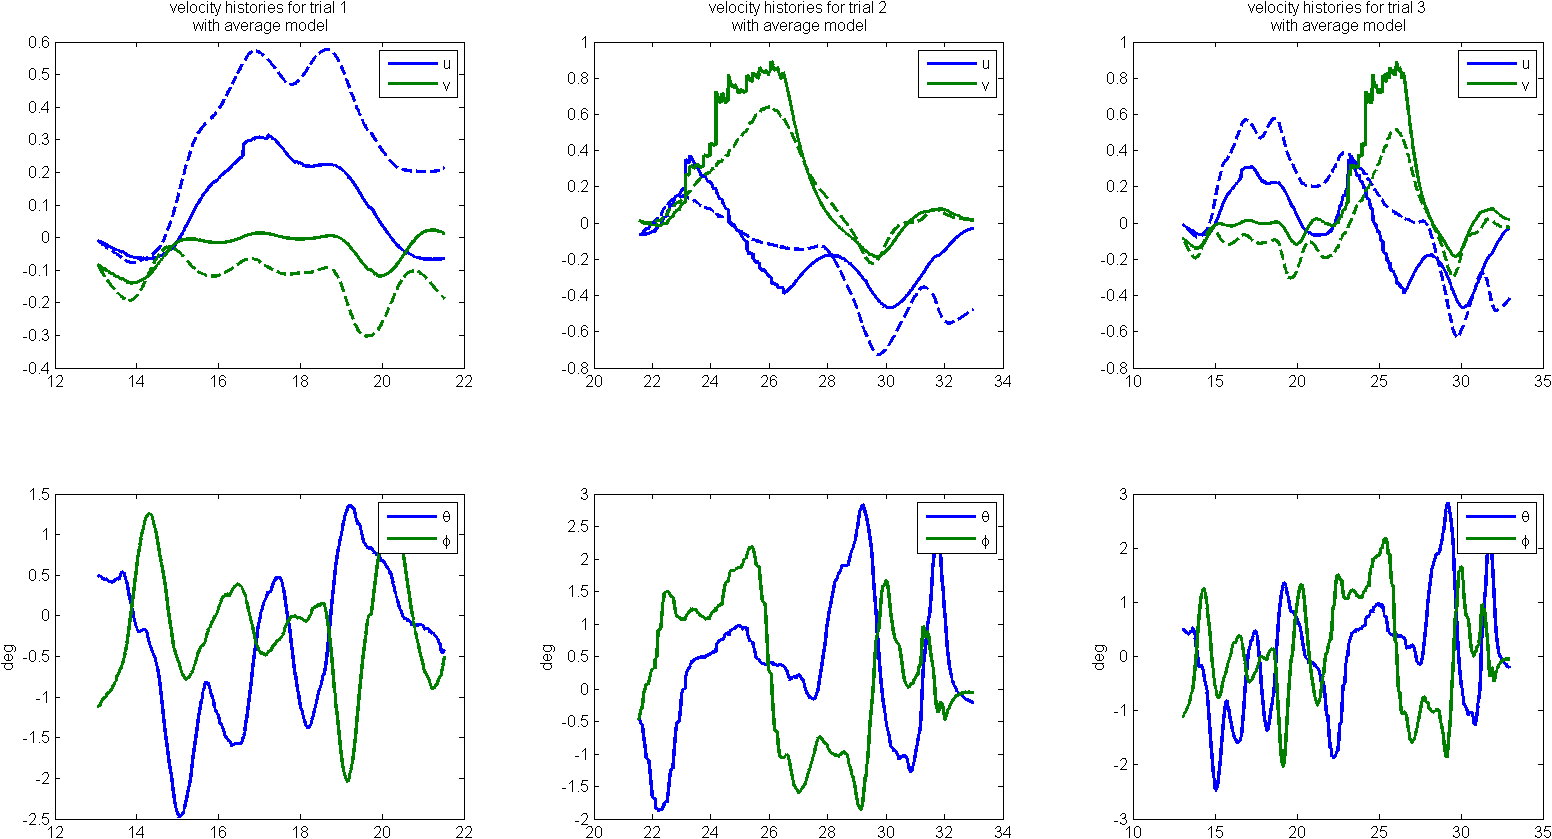
\includegraphics[width = \textwidth]{../../near system identification/model_day_1.png}
\caption{Plots of measured outputs (solid lines) and model-predicted outputs (dashed lines) for day 1 data. Upper charts show state (velocity) histories; lower charts show measured attitude for reference.}
\label{fig:day1mse}
\end{figure}

\begin{figure}[tb!]
\centering
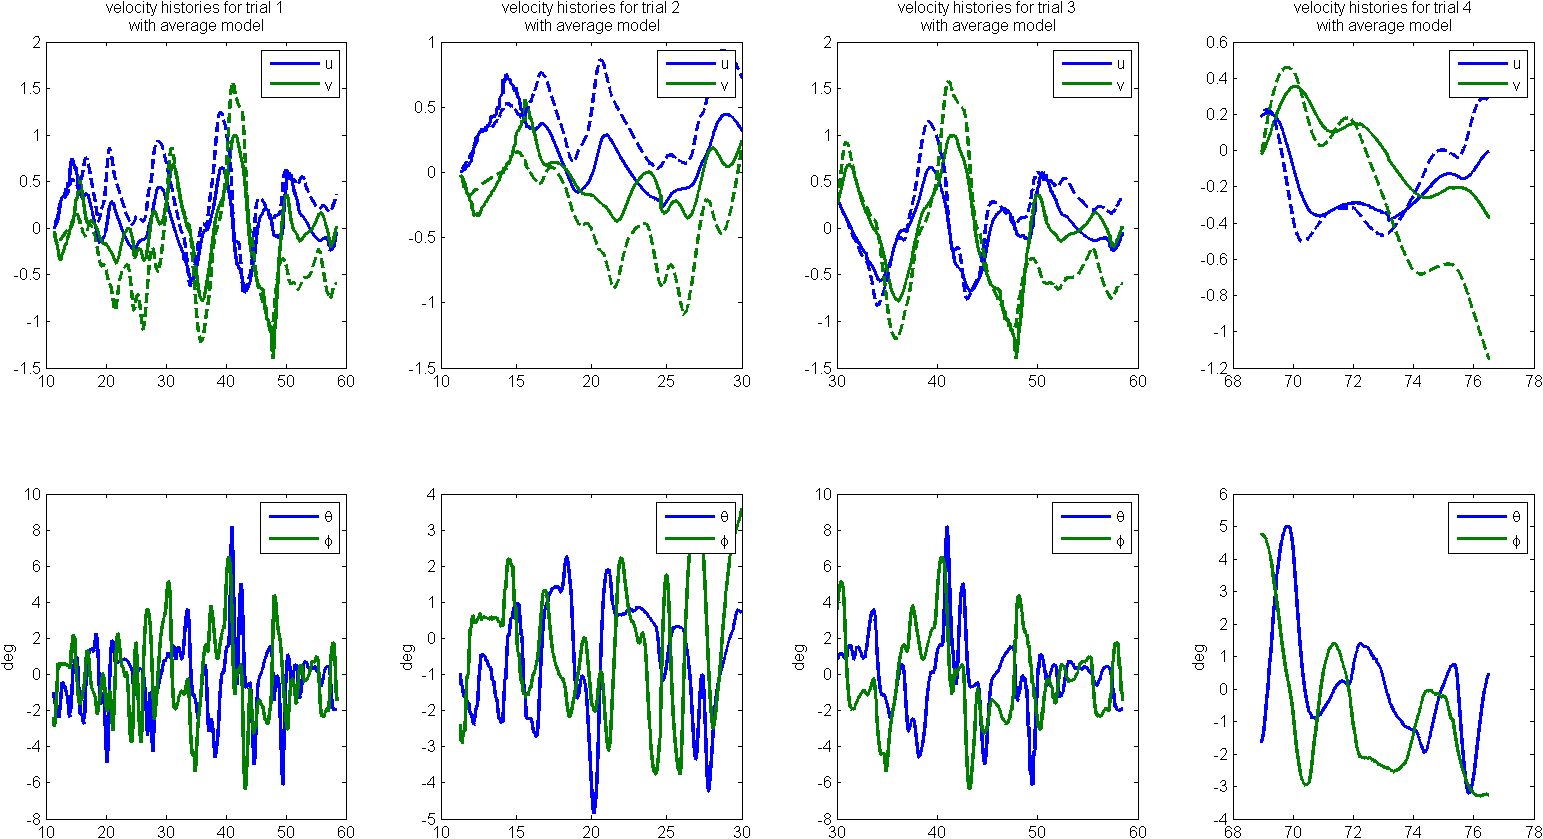
\includegraphics[width = \textwidth]{../../near system identification/model_day_2.png}
\caption{Plots of measured outputs (solid lines) and model-predicted outputs (dashed lines) for day 2 data. Upper charts show state (velocity) histories; lower charts show measured attitude for reference.}
\label{fig:day2mse}
\end{figure}

\subsection{Sensor characterization}

The objective of sensor characterization is to obtain appropriate covariance values for Kalman filtering, as well as to provide more accurate models for closed-loop control simulation. Covariance terms are required for the accelerometer, gyroscope, and optic flow sensor range and velocity measurements. In addition, some estimate of the gyroscope bias drift rate is required. The optimal estimate of the sensor variances is simply the standard deviation of errors with respect to Optitrack measurements; however, this is under the assumption that the measurements are actually Gaussian. The situation is further complicated when the potential for errors in the Optitrack data is acknowledged.

In an effort to obtain realistic yet conservative noise levels, the accelerometers and gyroscopes are characterized by hovering the vehicle in a position hold flight mode. This approach admits some excess uncertainty due to the vehicle's motion; however, it allows the effect of structural vibration due to the rotors to be included in the modelled variance, and should largely avoid the need to address potential Optitrack errors (in the acceleration term especially). 

Initial results using the optic flow sensors indicate that the velocity estimate from this sensor tracks the truth value only when the velocities are excited above a deadband of approximately 0.2 m/s. It is appropriate to characterize the typical returns in hovering flight, but the sensor variance in the presence of motion must also be characterized. This is achieved by flying the vehicle in position hold mode (an augmented manual flight mode) at varying altitudes and speeds, and comparing against truth measurements from Optitrack. 

Two primary checks are performed on measurement errors. First, a histogram of the errors should appear Gaussian or, if not Gaussian, should be symmetric and have a sharper peak than a normal distribution, such that Gaussian error bounds are somewhat conservative. This consideration is largely qualitative, but is quantitatively verified by testing that the number of measurements outside the $3\sigma$ bounds is on the order of 1\%. Second, a plot of errors as a function of the measured value should have a slope of zero if the errors are purely Gaussian. More realistically, a linear fit of errors to measurements should have a slope of 10\degree or less.

Fig. \ref{fig:restaccelhist} shows histogram of accelerometer measurements during a thirty-second hovering flight. The data appear reasonably Gaussian, and the fraction of outliers is approximately 0.2\%. Table \ref{tab:acc} compares the mean and standard deviation of accelerometer measurements in hovering flight and at rest before and after flight. The standard deviations in flight are approximately 1.5 times those at rest; the mean values do not vary greatly. Conservatively, a factor of 1.5 times the measured standard deviation in flight is taken as the accelerometer standard deviation, so the final values are:

\begin{equation}
\sigma_X,\sigma_Y,\sigma_Z = 0.84,0.81,0.54 \ \mathrm{m/s^2}
\end{equation}

\begin{figure}[tb!]
\centering
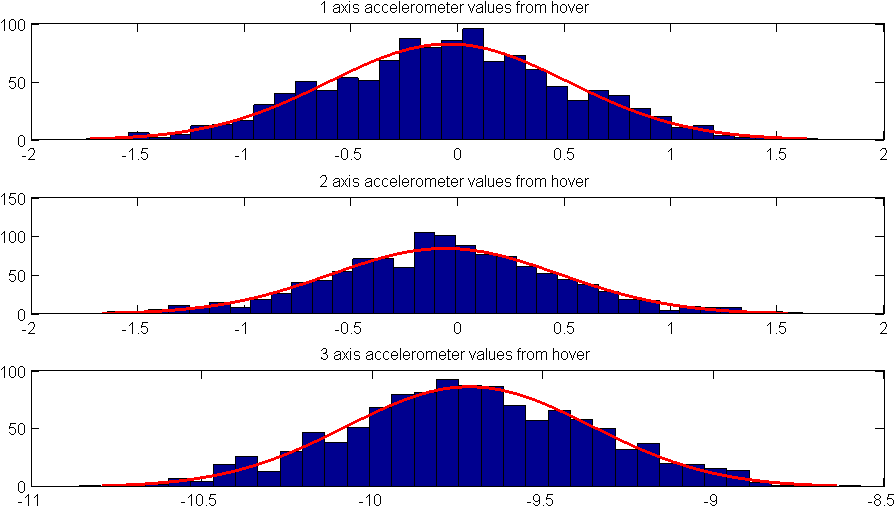
\includegraphics[width = \textwidth]{../../sensor characterization/rest_accel_hist.png}
\caption{Histogram of accelerometer returns with normal distribution best-fit curve.}
\label{fig:restaccelhist}
\end{figure}

\begin{table}[tb!]
\begin{tabular}{c|c|c|c|c|c|c}
Flight segment & $\mu_X$ & $\mu_Y$ & $\mu_Z$ & $\sigma_X$ & $\sigma_Y$ & $\sigma_Z$\\
Rest 1 & -0.045 & -0.10 & -9.7 & 0.34 & 0.31 &  0.20\\
Rest 2 & -.037 & -.15 & -9.7 & 0.37 & 0.39 & 0.24\\
Hover & -.045 & -.059 & -9.7 & 0.56 & 0.54 & 0.36\\
\end{tabular}
\caption{Comparison of accelerometer measurements at rest and in hovering flight.}
\label{tab:acc}
\end{table}

Similar results will be generated for the gyroscope errors. For the optic flow errors, the standard deviation of measurements at rest and in motion will be determined. Typical bias levels will be estimated by comparing mean errors across multiple flights.

\section{Summary}

\printbibliography

\end{document}
